\documentclass[a4paper,11pt]{article}
\usepackage[utf8]{inputenc}
\usepackage[spanish]{babel}
\usepackage[affil-it]{authblk}
\usepackage{enumerate}
\usepackage{graphicx}
\usepackage{listings}
\usepackage{hyperref}
\usepackage{amsmath}
\usepackage{amssymb}
\usepackage{cancel}
\usepackage[usenames, dvipsnames]{color}
\usepackage{tikz}
\usepackage[labelfont=bf]{caption}
\usepackage{subcaption} %Multiple images
\usepackage{multicol} % Multiple columns
\usepackage{float}
\usepackage{cleveref}
\usepackage{relsize} % bigger math symbols
\usepackage[margin=1.1in]{geometry}
\usepackage[titletoc,toc,title]{appendix}
\usepackage{enumitem}
\usepackage{etoolbox}
\usepackage{mdframed} %frame theorems
\usetikzlibrary{calc}
\numberwithin{equation}{section}

% Footnotes with symbols

\makeatletter
\def\@fnsymbol#1{\ensuremath{\ifcase#1\or \dagger\or \ddagger\or
   \mathsection\or \mathparagraph\or \|\or **\or \dagger\dagger
   \or \ddagger\ddagger \else\@ctrerr\fi}}
\makeatother

\renewcommand{\thefootnote}{\fnsymbol{footnote}}

%Styling for code
\definecolor{codegreen}{rgb}{0,0.6,0}
\definecolor{codegray}{rgb}{0.5,0.5,0.5}
\definecolor{codepurple}{rgb}{0.58,0,0.82}
\definecolor{backcolour}{rgb}{0.95,0.95,0.92}
 
\lstdefinestyle{mystyle}{
    backgroundcolor=\color{backcolour},   
    commentstyle=\color{codegreen},
    keywordstyle=\color{magenta},
    numberstyle=\tiny\color{codegray},
    stringstyle=\color{codepurple},
    basicstyle=\footnotesize,
    breakatwhitespace=false,         
    breaklines=true,                 
    captionpos=b,                    
    keepspaces=true,                 
    numbers=left,                    
    numbersep=5pt,                  
    showspaces=false,                
    showstringspaces=false,
    showtabs=false,                  
    tabsize=2
}
 
\lstset{style=mystyle}

% Cool letters 
%Filename:      Typocaps.fd
%Created by:    MLO
%Creation date: 2003/04/02

% This file should be put in a TeX input directory

\ProvidesFile{Typocaps.fd}
   [2003/04/02 Font definition file for U/Typocaps]

\DeclareFontFamily{U}{Typocaps}{}

\DeclareFontShape{U}{Typocaps}{xl}{n}{
   <-> Typocaps
}{}

\endinput


% Footer
\usepackage{fancyhdr}
\pagestyle{fancy}
\fancyhf{}
\cfoot{\fontsize{15pt}{15pt}\usefont{U}{Typocaps}{xl}{n} 
gigantium humeris insidentes}

% Big Pictures
\usepackage[export]{adjustbox}

% Enviroment for theorems
\newmdtheoremenv[frametitle=Teorema]{theo}{Theorem}

% Circled words
\newcommand{\circled}[2][]{%
  \tikz[baseline=(char.base)]{%
    \node[shape = circle, draw, inner sep = 1pt]
    (char) {\phantom{\ifblank{#1}{#2}{#1}}};%
    \node at (char.center) {\makebox[0pt][c]{#2}};}}
\robustify{\circled}

%Appendices in spanish
\renewcommand{\appendixname}{Ap\'endices}
\renewcommand{\appendixtocname}{Ap\'endices}
\renewcommand{\appendixpagename}{Ap\'endices}

%Zero delimiter
\newcommand{\zerodel}{.\kern-\nulldelimiterspace}

%Columns separation
\setlength{\columnsep}{1cm}

%Indentation
\setlength{\parindent}{0ex}

%Multiple References

\crefrangelabelformat{equation}{(#3#1#4--#5\crefstripprefix{#1}{#2}#6)}

\usepackage{xparse}

%Boxes

\newcommand*{\boxcolor}{blue}
\makeatletter
\renewcommand{\boxed}[1]{\textcolor{\boxcolor}{%
\tikz[baseline={([yshift=-1ex]current bounding box.center)}] \node [rectangle, minimum width=1ex,rounded corners,draw] {\normalcolor\m@th$\displaystyle#1$};}}
 \makeatother

%Constantes
\newcommand{\euler}{\mathrm{e}}
\newcommand{\im}{i}

%Lemas, teoremas, definiciones y pruebas
\newcommand{\definicion}{\textbf{Definición: }}
\newcommand{\lema}{\textbf{Lema: }}
\newcommand{\teorema}{\textbf{Teorema: }}
\newcommand{\prueba}{\textbf{Prueba: }}
\newcommand{\proposicion}{\textbf{Proposición: }}
\newcommand{\corolario}{\textbf{Corolario: }}

% Definición de las secciones y su numeración

\makeatletter
\def\@seccntformat#1{%
  \expandafter\ifx\csname c@#1\endcsname\c@section\else
  \csname the#1\endcsname\quad
  \fi}
\makeatother

\begin{document}

\begin{titlepage}
\thispagestyle{fancy}

\newcommand{\HRule}{\rule{\linewidth}{0.5mm}} % Defines a new command for the horizontal lines, change thickness here

\center % Center everything on the page
 
%----------------------------------------------------------------------------------------
%	HEADING SECTIONS
%----------------------------------------------------------------------------------------

\textsc{\LARGE Universidad Nacional Autónoma de México}\\[0.3cm] % Name of your university/college

%----------------------------------------------------------------------------------------
%	LOGO SECTION
%----------------------------------------------------------------------------------------


\includegraphics[scale=0.17]{unam}

%----------------------------------------------------------------------------------------
%	SUBHEADING SECTIONS
%----------------------------------------------------------------------------------------

\textsc{\Large Electrodinámica Clásica}\\[0.3cm] % Major heading such as course name
\textsc{\large Semestre 2016-II}\\[0.3cm] % Minor heading such as course title
\textsc{\large 5 de mayo de 2016}\\ % Date

%----------------------------------------------------------------------------------------
%	TITLE SECTION
%----------------------------------------------------------------------------------------

\HRule \\[0.1cm]
{ \huge \bfseries Tarea \# 8. \\ Deducción de los campos eléctricos y magnéticos de velocidad y 
aceleración a partir de los potenciales de Lienard-Wiechert.}\\ % Title of your document
\HRule \\[0.1cm]
 
%----------------------------------------------------------------------------------------
%	AUTHOR SECTION
%----------------------------------------------------------------------------------------
\setcounter{footnote}{0}
\center
\large
\emph{Autor:} \\ % Your name
\Large Favio \textsc{Vázquez}\footnote[1]{\href{mailto:favio.vazquez@correo.nucleares.unam.mx}{favio.vazquez@correo.nucleares.unam.mx}}
\\[0.7cm]
%----------------------------------------------------------------------------------------
%	COOL IMAGE SECTION
%----------------------------------------------------------------------------------------

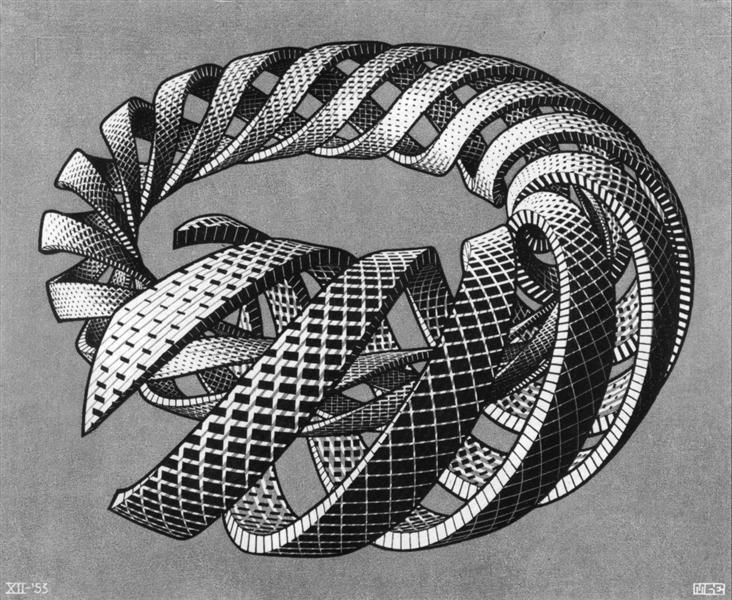
\includegraphics[scale=0.55]{escherEspiral}

%----------------------------------------------------------------------------------------

\vfill % Fill the rest of the page with whitespace

\end{titlepage}

% ---------------------------------------------------------------------------------------
%         HEADER
%----------------------------------------------------------------------------------------

\fancyhead[L]{Favio Vázquez}
\fancyhead[R]{\thepage}

%----------------------------------------------------------------------------------------
\setcounter{footnote}{0}
\renewcommand*{\thefootnote}{\arabic{footnote}}
%----------------------------------------------------------------------------------------

%----------------------------------------------------------------------------------------
%%			BEGIN DOCUMENT
%----------------------------------------------------------------------------------------

\section{Diferenciación de los potenciales de Lienard-Wiechert.}

Esta deducción se hizo siguiendo los resultados de las secciones 6.2 y 6.3 del 
libro de Schwartz \cite{schwartz}. Los potenciales de Lienard-Wiechert podemos 
escribirlos como 

\begin{equation}
 \phi(\mathbf{r},t) = \frac{q}{|\mathbf{r}-\mathbf{r}'(t')\left[1 - 
 \frac{v'(t')\cdot \hat{\mathbf{\epsilon}}}{c}\right]},
\end{equation}

y 

\begin{equation}
 \mathbf{A}(\mathbf{r},t) = \frac{q\mathbf{v}'(t')}{c|\mathbf{r}-\mathbf{r}'(t')\left[1 - 
 \frac{v'(t')\cdot \hat{\mathbf{\epsilon}}}{c}\right]},
\end{equation}

donde $q$ es la carga de la partícula, $\mathbf{v}(t)$ y $\mathbf{\epsilon}$ 
es un vector unitario de $\mathbf{r}'(t')$ a $\mathbf{r}$, 

\begin{equation}
 \mathbf{\epsilon}' = \frac{\mathbf{r}-\mathbf{r}'(t')}{|\mathbf{r}-\mathbf{r}'(t')|}.
\end{equation}

Podemos pasar ahora a calcular ahora los campos eléctricos y magnéticos debidos a 
nuestras pequeñas cargas en movimiento. Aunque en el régimen no relativista, nos 
interesan situaciones donde $v \ll c$, trabajaremos por el momento manteniendo 
todos los órdenes en $v/c$. Nuestro trabajo se convierte entonces en diferenciar 
estos potenciales, para encontrar 

\begin{equation}
 \mathbf{B}(\mathbf{r},t) = 
 \pmb{\nabla} \times \frac{q\mathbf{v}'(t')}{c|\mathbf{r}-\mathbf{r}'(t')\left[1 - 
 \frac{v'(t')\cdot \hat{\mathbf{\epsilon}}}{c}\right]},
\end{equation}

\begin{equation}
 \mathbf{E}(\mathbf{r},t) = - \pmb{\nabla}  \frac{q}{|\mathbf{r}-\mathbf{r}'(t')\left[1 - 
 \frac{v'(t')\cdot \hat{\mathbf{\epsilon}}}{c}\right]} - \frac{1}{c} 
 \frac{\partial}{\partial t}\left[\frac{q\mathbf{v}'(t')}{c|\mathbf{r}-\mathbf{r}'(t')\left[1 - 
 \frac{v'(t')\cdot \hat{\mathbf{\epsilon}}}{c}\right]} \right].
\end{equation}

La dificultad de estas derivaciones yace en la compleja dependencia implícita 
de los términos primados en $\mathbf{r}$ y $t$. Definiendo el tiempo retardado 
como 

\begin{equation}
 t' = t - \frac{|\mathbf{r} - \mathbf{r}'|}{c},
\end{equation}

entonces 

\begin{equation}
 \frac{\partial t'}{\partial t} = 1 - \frac{1}{c}\left(\frac{\partial}{\partial t'}
 |\mathbf{r} - \mathbf{r}'|\right)\frac{\partial t'}{\partial t},
\end{equation}

y

\begin{equation}
 \frac{\partial |\mathbf{r} - \mathbf{r}'|}{\partial t'} = - \mathbf{v}' \cdot 
 \hat{\mathbf{\epsilon}}',
\end{equation}

por lo tanto

\begin{equation}
 \frac{\partial t'}{\partial t} = \frac{1}{1 - \frac{\mathbf{v}' \cdot \mathbf{\epsilon}'}{c}}.
\end{equation}

Similarmente, 

\begin{equation}
 \nabla t' = \frac{1}{c}\hat{\mathbf{\epsilon}}' - 
 \frac{1}{c}\left(\frac{\partial}{\partial t'}|\mathbf{r} - \mathbf{r}'|\right)
 \nabla t',
\end{equation}

y entonces 

\begin{equation}
 \nabla t' = \frac{- \hat{\mathbf{\epsilon}}'}{c\left(1 - \frac{\mathbf{v}' 
 \cdot \hat{\mathbf{\epsilon}}}{c} \right)}.
\end{equation}

También será útil el siguiente resultado:

\begin{equation}
 \frac{\partial \hat{\mathbf{\epsilon}}'}{\partial t'} = 
 \frac{\partial}{\partial t'}\left(\frac{\mathbf{r} - \mathbf{r}'}{|\mathbf{r} - \mathbf{r}'|}\right) = 
 \frac{(\mathbf{v}' \cdot \hat{\mathbf{\epsilon}}'(\mathbf{r} - \mathbf{r}')}{|\mathbf{r} - \mathbf{r}'|^2} 
 - \frac{\mathbf{v}'}{|\mathbf{r} - \mathbf{r}'|}.
\end{equation}

o 

\begin{equation}
 \frac{\partial \hat{\mathbf{\epsilon}}'}{\partial t'} = \frac{\hat{\mathbf{\epsilon}}' 
 \times (\hat{\mathbf{\epsilon}}' \times \mathbf{v}')}{|\mathbf{r} - \mathbf{r}'|}.
\end{equation}

Podemos evaluar 

\begin{equation*}
 \frac{\partial}{\partial t'}\left[|\mathbf{r} - \mathbf{r}'| \left(1 - 
 \frac{\mathbf{v}| \cdot  \hat{\mathbf{\epsilon}}'}{c}\right) \right] = 
 - \mathbf{v}| \cdot  \hat{\mathbf{\epsilon}}' \left(1 - 
 \frac{\mathbf{v}' \cdot  \hat{\mathbf{\epsilon}}'}{c}\right) - 
 |\mathbf{r} - \mathbf{r}'|\frac{\mathbf{a}'}{c}\cdot \hat{\mathbf{\epsilon}}' 
 - \frac{\mathbf{v}'}{c}\cdot \left[\hat{\mathbf{\epsilon}}' \times
 (\hat{\mathbf{\epsilon}}' \times \mathbf{v}')\right]
\end{equation*}

o

\begin{equation}
  \frac{\partial}{\partial t'}\left[|\mathbf{r} - \mathbf{r}'| \left(1 - 
 \frac{\mathbf{v}| \cdot  \hat{\mathbf{\epsilon}}'}{c}\right) \right] = 
 \frac{-|\mathbf{r} - \mathbf{r}'|\mathbf{a}' \cdot \hat{\mathbf{\epsilon}}'}{c} 
 - \mathbf{v}' \cdot \hat{\mathbf{\epsilon}}' + \frac{v'^2}{c},
\end{equation}

que nos da 

\begin{equation}
  \frac{\partial}{\partial t'}\left[|\mathbf{r} - \mathbf{r}'| \left(1 - 
 \frac{\mathbf{v}| \cdot  \hat{\mathbf{\epsilon}}'}{c}\right) \right] = 
 \frac{-|\mathbf{r} - \mathbf{r}'|\mathbf{a}' \cdot \hat{\mathbf{\epsilon}}'}{c} 
 - \mathbf{v}| \cdot \left(\hat{\mathbf{\epsilon}}' - \frac{\mathbf{v}'}{c} \right),
\end{equation}

donde 

\begin{equation}
 \mathbf{a}' = \frac{d\mathbf{v}'}{dt'}.
\end{equation}

Estamos listos ahora para encontrar el gradiente de $\phi$, 

\begin{equation}
 - \nabla \phi = - (\nabla \phi)_{t'const} - \frac{\partial \phi}{\partial t'}
 \nabla t',
\end{equation}

al hacer estos cálculos encontramos 

\begin{equation}
 - \nabla \phi = \frac{q\left[\hat{\mathbf{\epsilon}}' \left(1 - 
 \frac{v'^2}{c^2}\right) - \frac{\mathbf{v}'}{c}\left(1 - \frac{v}{c}\cdot 
 \hat{\mathbf{\epsilon}}'\right) \right]}{|\mathbf{r} - \mathbf{r}'| 
 \left(1 - \frac{\mathbf{v}' \cdot \hat{\mathbf{\epsilon}}'}{c}\right)^3} 
 + \frac{q\hat{\mathbf{\epsilon}}'(\mathbf{a}' \cdot \hat{\mathbf{\epsilon}}')}{ 
 c^2|\mathbf{r} - \mathbf{r}'|\left(1 - \frac{\mathbf{v}' \cdot 
 \hat{\mathbf{\epsilon}}'}{c} \right)^3}.
\end{equation}

Ahora calculamos 

\begin{equation}
 - \frac{1}{c}\frac{\partial\mathbf{A}}{\partial t} = - \frac{1}{c} 
 \frac{\partial \mathbf{A}}{\partial t'}\frac{\partial t'}{\partial t},
\end{equation}

\begin{equation}
 - \frac{1}{c}\frac{\partial\mathbf{A}}{\partial t} = - \frac{\partial}{\partial t'} 
 \frac{q\mathbf{v}'}{c^2|\mathbf{r} - \mathbf{r}'|\left(1 - \frac{\mathbf{v}' 
 \cdot \hat{\mathbf{\epsilon}}'}{c} \right)},
\end{equation}

y al hacer la derivada obtenemos (y con un poco de álgebra)

\begin{equation}
 - \frac{1}{c}\frac{\partial\mathbf{A}}{\partial t} = \frac{-q \frac{\mathbf{v}'}{c} 
 \left[\frac{\mathbf{v}'}{c} \cdot \left(\hat{\mathbf{\epsilon}}' - 
 \frac{\mathbf{v}'}{c}\right)\right]}{|\mathbf{r} - \mathbf{r}'|^2 
 \left(1 - \frac{\mathbf{v}'\cdot \hat{\mathbf{\epsilon}}'}{c} \right)^3} + 
 \frac{-q\mathbf{a}' + q\hat{\mathbf{\epsilon}}' \times \left(\mathbf{a}' 
 \times \frac{\mathbf{v}'}{c}\right)}{c^2|\mathbf{r} - \mathbf{r}'|
  \left(1 - \frac{\mathbf{v}'\cdot \hat{\mathbf{\epsilon}}'}{c} \right)^3}
\end{equation}

Combinando $- \nabla \phi$ y $- \frac{1}{c}\frac{\partial A}{\partial t}$, podemos 
calcular el campo eléctrico que queda como 

\begin{equation}
 \boxed{\mathbf{E}(\mathbf{r},t) = \frac{-q[\mathbf{a}' - (\mathbf{a}' \cdot 
 \hat{\mathbf{\epsilon}}')\hat{\mathbf{\epsilon}}' + q\hat{\mathbf{\epsilon}}' 
 \times \left(\mathbf{a}' \times \frac{\mathbf{v}'}{c} \right)]}{c^2 
 |\mathbf{r} - \mathbf{r}'|\left(1 - \frac{\mathbf{v}'\cdot 
 \hat{\mathbf{\epsilon}}'}{c} \right)^3} + 
 \frac{q \left(\hat{\mathbf{\epsilon}}' - \frac{\mathbf{v}'}{c} \right)\left( 
 1 - \frac{v'^2}{c^2}\right)}{|\mathbf{r} - \mathbf{r}'|^2 
  \left(1 - \frac{\mathbf{v}'\cdot \hat{\mathbf{\epsilon}}'}{c} \right)^3}}.
\end{equation}

Ahora, calculamos el campo magnético con $\mathbf{B} = \pmb{\nabla} \times \mathbf{A}$, 

\begin{equation}
 \pmb{\nabla} \times \mathbf{A} = ( \pmb{\nabla} \times \mathbf{A})_{t'const} - 
 \left(\frac{\mathbf{A}}{\partial t'} \right) \nabla t'.
\end{equation}

Entonces, 

\begin{equation}
  ( \pmb{\nabla} \times \mathbf{A})_{t'const} = \frac{-q\left(\hat{\mathbf{\epsilon}}' 
  - \frac{\mathbf{v}'}{c}\right) \times \frac{\mathbf{v}'}{c}}{|\mathbf{r} - \mathbf{r}'|^2 
  \left(1 - \frac{\mathbf{v}'\cdot \hat{\mathbf{\epsilon}}'}{c} \right)^2},
\end{equation}

y 

\begin{equation}
 - \frac{\partial \mathbf{A}}{\partial t'} \times \nabla t' = 
 \frac{q\mathbf{a}' \times  \hat{\mathbf{\epsilon}}' + 
 q \hat{\mathbf{\epsilon}}' \times \left[ \hat{\mathbf{\epsilon}}' \times 
 \left(\mathbf{a}' \times \frac{\mathbf{v}'}{c} \right)\right]}{c^2 
 |\mathbf{r} - \mathbf{r}'|\left(1 - \frac{\mathbf{v}'\cdot 
 \hat{\mathbf{\epsilon}}'}{c} \right)^3} + 
 \frac{q\left(\frac{\mathbf{v}'}{c} \times \hat{\mathbf{\epsilon}}' \right)
 \left[\frac{\mathbf{v}'}{c} \cdot \left(\hat{\mathbf{\epsilon}}' - 
 \frac{\mathbf{v}'}{c}\right) \right]}{|\mathbf{r} - \mathbf{r}'|^2\left(1 - \frac{\mathbf{v}'\cdot 
 \hat{\mathbf{\epsilon}}'}{c} \right)^3},
\end{equation}

y finalmente tenemos 

\begin{equation}
 \boxed{\mathbf{B} = \frac{q\left(\frac{\mathbf{v}'}{c} \times \hat{\mathbf{\epsilon}}'\right) 
 \left(1 - \frac{v'^2}{c^2}\right)}{|\mathbf{r} - \mathbf{r}'|^2\left(1 - \frac{\mathbf{v}'\cdot 
 \hat{\mathbf{\epsilon}}'}{c} \right)^3} + \hat{\mathbf{\epsilon}}' \times 
 \frac{-q\mathbf{a}' + q\left[\hat{\mathbf{\epsilon}}' \times 
 \left(\mathbf{a}' \times \frac{\mathbf{v}'}{c} \right) \right]}{c^2|\mathbf{r} - \mathbf{r}'|
 \left(1 - \frac{\mathbf{v}'\cdot  \hat{\mathbf{\epsilon}}'}{c} \right)^3}}.
\end{equation}

Si examinamos las expresiones que obtuvimos para $\mathbf{E}$ y $\mathbf{B}$, notamos 
que cada una de ellas se divide naturalmente en dos partes, una que es independiente de 
la aceleración y decrece con $1/|\mathbf{r} - \mathbf{r}'|^2$ (campo de velocidad) 
y otra que es proporcional a la aceleración de la carga que decrece con 
$1/|\mathbf{r} - \mathbf{r}'|$ (campo de aceleración). Los términos proporcionales a 
$\mathbf{a}$ son los que nos interesan, y son los llamados campos de radiación. 

\begin{thebibliography}{10}
\bibitem{schwartz}
 M. Schwartz, \emph{Principles of electrodynamics}, Dover Publications, Inc. 1972.
\end{thebibliography}

\end{document}